\documentclass[12pt, letterpaper]{article}
\usepackage[titletoc,title]{appendix}
\usepackage{color}
\usepackage{booktabs}
\usepackage[usenames,dvipsnames,svgnames,table]{xcolor}
\definecolor{dark-red}{rgb}{0.75,0.10,0.10} 
\usepackage[margin=1in]{geometry}
\usepackage[linkcolor=dark-red,
            colorlinks=true,
            urlcolor=blue,
            pdfstartview={XYZ null null 1.00},
            pdfpagemode=UseNone,
            citecolor={dark-red},
            pdftitle={Typecast: A Routine Mental Shortcut Causes Party Stereotyping}]{hyperref}

\usepackage[resetlabels,labeled]{multibib}
\newcites{SI}{SI References}
\usepackage{natbib}
\usepackage[section]{placeins}
\usepackage{float}

\usepackage{geometry} % see geometry.pdf on how to lay out the page. There's lots.
\geometry{letterpaper}               % This is 8.5x11 paper. Options are a4paper or a5paper or other... 
\usepackage{graphicx}                % Handles inclusion of major graphics formats and allows use of 
\usepackage{amsfonts,amssymb,amsbsy}
\usepackage{amsxtra}
\usepackage{verbatim}
\setcitestyle{round,semicolon,aysep={},yysep={;}}
\usepackage{setspace}             % Permits line spacing control. Options are \doublespacing, \onehalfspace
\usepackage{sectsty}             % Permits control of section header styles
\usepackage{lscape}
\usepackage{fancyhdr}             % Permits header customization. See header section below.
\usepackage{url}                     % Correctly formats URLs with the \url{} tag
\usepackage{fullpage}        %1-inch margins
\usepackage{multirow}
\usepackage{rotating}
\usepackage{comment}
\setlength{\parindent}{3em}

\usepackage[T1]{fontenc}
%\usepackage{bm}
\usepackage{libertine}

\usepackage{chngcntr}

%This section double-spaces & makes footnotes the same size as normal text.
%\usepackage{footmisc}
%\setlength{\footnotesep}{\baselineskip}
%\makeatother
%\renewcommand{\footnotelayout}{\normalsize \doublespacing}

% Alternative citation styles
\def\citeapos#1{\citeauthor{#1}'s (\citeyear{#1})}


% Caption
\usepackage[hang, font=small,skip=0pt, labelfont={bf}]{caption}
%\captionsetup[subtable]{font=small,skip=0pt}
\usepackage{subcaption}

% tt font issues
% \renewcommand*{\ttdefault}{qcr}
\renewcommand{\ttdefault}{pcr}

\setcounter{page}{0}

\usepackage{lscape}
\renewcommand{\textfraction}{0}
\renewcommand{\topfraction}{0.95}
\renewcommand{\bottomfraction}{0.95}
\renewcommand{\floatpagefraction}{0.40}
\setcounter{totalnumber}{5}
\makeatletter
\providecommand\phantomcaption{\caption@refstepcounter\@captype}
\makeatother

\title{Typecast: A Routine Mental Shortcut \\ Causes Party Stereotyping\footnote{We thank the American Politics \& Public Policy workshop at Yale University and the Political Behavior \& Identities workshop at Duke University for participants' helpful questions, thoughts, and suggestions. We also appreciate our fellow panelists at MPSA 2017 for their feedback. Stephen Goggin, Marcel Garz, Brad Gomez, Bob Jackson, Kabir Khanna, Matt Levendusky, Matt Pietryka, Carrie Roush, and Julie Wronski also offered helpful comments. We are grateful to them.}}

\author{Douglas J. Ahler\thanks{Doug is Assistant Professor of Political Science at the Florida State University, \href{mailto:dahler@fsu.edu}{\texttt{dahler@fsu.edu}}.} \and Gaurav Sood\thanks{Gaurav can be reached at \href{mailto:gsood07@gmail.com}{\texttt{gsood07@gmail.com}}.}}

\begin{document}
\maketitle
\begin{center}
\textbf{Word count:}  8,907
\end{center}
\thispagestyle{empty}

\begin{abstract}

\noindent Party stereotyping inflames polarization. What fuels party stereotyping? We explore the extent to which a common mental shortcut---the representativeness heuristic---yields biased mental images of the parties. First, we show that people commit the conjunction fallacy---a logical error associated with representativeness bias---at higher rates when evaluating others with party-representative characteristics. Second, when we inform people of the percentage of partisans in groups, the least numerate use this information to infer party composition, consistent with the representativeness heuristic. Finally, we show that people's party stereotypes become more biased when we increase cognitive load, though stereotyping occurs even in relatively ``easy'' contexts. The representativeness heuristic appears to exacerbate party stereotyping, and the way that media informs people about the relationship between social groups and parties may encourage reliance on representativeness. More broadly, reducing stereotyping requires reckoning with our built-in machinery for simplifying the world around us.

%\noindent Party stereotyping inflames partisan polarization. What fuels party stereotyping? We explore the extent to which a common mental shortcut---the representativeness heuristic---yields biased mental images of the parties. First, we show that people commit the conjunction fallacy---a logical error associated with representativeness bias---at higher rates when evaluating others with party-representative characteristics. Second, when we provide group composition by party---$p(\text{party}|\text{group})$---people, especially the least numerate, use the latter to infer party composition, consistent with the representativeness heuristic. When we provide base rates---$p(\text{group}$)---some offer slightly more accurate estimates, but the least numerate's perceptions remain as biased. Finally, we show that people's perceptions of party composition become more biased toward $p(\text{party}|\text{group})$ when we increase cognitive load, though stereotyping occurs even in relatively ``easy'' contexts. The representativeness heuristic appears to exacerbate party stereotyping. More broadly, reducing stereotyping requires reckoning with our built-in machinery for simplifying the world around us. 

%Party stereotyping fuels partisan polarization. People hold biased beliefs about what the parties look like and when these misperceptions are corrected, they feel warmer toward the other side (Ahler and Sood 2018). But what fuels party stereotyping itself? We demonstrate the automaticity of party stereotyping and then explore the extent to which a common mental shortcut---the representativeness heuristic---leads to biased mental images of the parties. First, through a series of experiments based on ``the Linda problem'' (Tversky and Kahneman 1983), we show that when people see party-representative characteristics in others, they are liable to commit the conjunction fallacy---a logical error associated with representativeness bias. Second, through an experiment priming base rates---$p(\text{group})$---and group composition by party---$p(\text{party}|\text{group})$---we show that people, especially the least numerate, use the latter to infer party composition, consistent with a reliance on representativeness. When we provide base rates, people offer somewhat more accurate estimates, but the least numerate's perceptions remain as biased. Finally, we show that people's perceptions of party composition become more biased toward $p(\text{party}|\text{group})$ when we increase cognitive load through time pressure. These studies demonstrate that people's reliance on the representativeness heuristic exacerbates party stereotyping. More broadly, reducing stereotyping requires a reckoning with our built-in machinery for simplifying the world around us.

\end{abstract}

\begin{comment}

setwd(paste0(githubdir, "typecast/ms/"))
tools::texi2dvi("typecast.tex", pdf = TRUE, clean = TRUE)
setwd(githubdir)

\end{comment}

\newpage
\doublespacing

\noindent Democrats and Republicans appear to be today's Montagues and Capulets---partisans from both sides of the aisle dislike each other to the point of rejecting inter-party marriage \citep[e.g.,][]{IyengarSoodLelkes2012, pew_polarization}. More broadly, both groups readily discriminate against each other, even when it is costly for them to do so \citep{IyengarWestwood2014, mcconnell2018economic}. This animus causes more harm than the mere provocation of tybaltian tempers---it appears to color partisans' political judgments. Notably, partisans increasingly distrust governments led by the opposing party, which hinders effective governance \citep{hetherington2015washington}.

One source of this animus is party stereotyping. Most Americans hold skewed mental images of Democrats and Republicans, vastly overestimating how common party-stereotypical groups are in ``their'' parties. For example, the median American thinks that 30\% of Republicans earn over \$250,000 per year---the actual percentage is no more than 4\% \citep{ahler2018parties}. Clearing up such misinformation reduces partisan animus \citep{ahler2018parties}.

But what explains stereotyping? The concept itself has been fundamental to the study of public opinion and political behavior for nearly a century---citizens' judgments often rely on simplications of their environments \citep[e.g.,][]{Lippmann1922, edwards1940four}. For example, party stereotypes structure people's understanding of day-to-day politics. Citizens infer candidates' policy positions from purely symbolic information about their partisanship \citep{goggin2017disputed, lodge1986partisan, Rahn1993}. They further use partisan stereotypes to make inferences about other citizens, often drawing hyperbolic distinctions---for example, overestimating differences in policy positions \citep{LevenduskyMalhotra2013} and moral values \citep{GrahamNosekHaidt2012} between people on the left and right. Beyond partisanship, the perniciousness of stereotyping is even more apparent. Racial stereotypes predict support for segregationist policies, anti-miscegenation laws, opposition to programs designed to lift Blacks out of poverty, and opposition to social welfare programs more generally \citep{carmines2011on, ditonto2013AMPing, gilens1995racial, gilens1996poq, gilens1996race, peffley1997racial, sniderman1993scar}. More recently, researchers have discovered that Americans tend to reduce the war on terrorism to a conflict between Christianity and Islam, and that over-attribution of violent attitudes to Muslims is commonplace \citep{tessler2003arab}, and that Americans with the most negative stereotypes about Muslims hold the most hawkish attitudes \citep{sides2013stereotypes}. By the same token, gender appears to structure the entire process by which people evaluate candidates for office---not only do partisans prefer candidates who comport to particular gender stereotypes \citep{bernhard2019wearing}, but citizens also tend to infer policy positions from candidate gender \citep{ditonto2014gender}. People even use distinct, gender-stereotypical information search processes when learning about male and female candidates \citep{huddy1993gender}. In sum, stereotypes appear to structure much of people's reasoning about politics.\footnote{It's worth noting the likely power of party stereotypes, race and gender stereotypes, and other stereotypes based on identities that are extremely consequential. In the case of party stereotypes, most Americans have one of these identities, which color how they tend to see the world \citep[e.g.][]{bartels2000} It's also worth noting that partisan stereotypes have strong valences---people dislike each other across party lines, and stereotypes tend to reflect groups that people do or do not like \citep{kane2021who}. Thus, party stereotyping may be a uniquely strong form of stereotyping.}

In this paper, we probe the hypothesis that \emph{representativeness bias}---the pattern of cognitive errors we make while using a fundamental judgment heuristic---drives political stereotyping. We explore this possibility in the context of contemporary party stereotyping. According to the \emph{group theory of parties}, people conceive of political parties in terms of longer standing groups in society \citep{ahler2018forum, busby2016what,GreenPalmquistSchickler2002,mason2018uncivil}. Since political parties are abstract---we can't literally meet the parties---we construct ``pictures in our heads'' from the available information \citep{Lippmann1922}. In doing so, we often use judgment shortcuts. Here, we show that one of these shortcuts in particular, the \emph{representativeness} heuristic, contributes greatly to people's biased maps of the political landscape. To rely on representativeness is to attend excessively to one's cognitive linkage between whatever is under consideration to a more general category (for example, the similarity between ``rich'' and ``Republican''), often to the detriment of other relevant factors (say, the proportion of people earning over \$250,000 in the U.S.). That is, people are swayed by the idea that ``like goes with like'' \citep{gilovich1981like}: even when that first ``like'' (the representative trait) is rare in the population, its similarity to the \emph{category prototype} leads people to overestimate its frequency within that category. In sum, instead of using Bayes's Rule and fully considering the percentage of the population that earns at least \$250,000 per year in addition to the percentage of those wealthy Americans who belong to the GOP, people focus almost exclusively on the latter, conflating $p($rich $|$ Republican$)$ with $p($Republican $|$ rich$)$. And, as a heuristic, people are liable to engage in this type of reasoning under higher levels of cognitive load and when representative characteristics of groups are especially salient.

People's beliefs about the parties are likely affected by many other factors, and this paper doesn't assert a mono-causal view on the roots of stereotypes. It merely explores the extent to which representativeness explains party stereotyping. In what follows, we develop testable hypotheses emerging from this idea, and then borrow and build on canonical designs from psychology that allow people to reveal their use of representativeness as a mental shortcut. Across six experiments, we find that people indeed use representativeness heuristically to construct the overly-stereotypical Democrats and Republicans in their heads. Potentially promisingly, we abate stereotyping in one of these experiments by requiring participants to take time to think through party composition. We conclude by noting that human cognition has a built-in machinery for reducing the world around us to stereotypes, but also that political media tends to present information about party-group linkages in a manner that encourages the use of the representativeness heuristic---and thus stereotyping.


\section{Representativeness and Stereotyping}

Stereotyping emerges in part from the necessity to take shortcuts. The world is complex and our cognitive capacity is limited---we cannot attend to even a small fraction of the details. \emph{Prototypes} are especially important for painting ``pictures in our heads'' \citep{Lippmann1922}. They exist in memory as agglomerations of the most central features of categories or groups \citep{RoschMervis1975} and help people quickly distinguish group members from non-members. Without cognitive structures like these, people couldn't function in the world. The constant bombardment of stimuli we receive would be overwhelming without being able to instinctively identify oranges as edible fruit, alligators as predators---and, for a variety of reasons, other humans as ``like us'' or not \citep{kinder2010us}, or of different status from us, as is the case with party stereotypes.

But how do particular characteristics and traits become prototypical? \citet{RoschMervis1975} assert that prototypicality stems not from differences in raw frequencies of types within broader categories, but rather from their \emph{relative} frequencies across categories. For example, when people think of African-Americans, basketball frequently comes to mind \citep{eberhardt2004seeing}. %\footnote{\citet{eberhardt2004seeing} further note the bidirectional thesis: subconsciously priming basketball leads people to think of African-Americans.} 
Across all racial groups in America, a minority of people play basketball. Further, fewer than half of NBA viewers are Black, and just a small minority of African-Americans watch NBA basketball routinely \citep{thompson2014which}. But African-Americans are relatively frequent among these groups---not only are about three-quarters of NBA players Black, but the NBA ``has the highest share of Black viewers (of all major sports leagues)---three times higher than the NFL or NCAA basketball'' \citep{thompson2014which}. Basketball is not universal in Black America, but it is stereotypical because it is relatively popular among Blacks vis-\`{a}-vis other racial groups.

This tendency to think distinguishing traits are common in groups is characteristic of the representativeness heuristic. Traits (e.g., ``Black'') that strongly predict membership in the category (in the example above, ``basketball fans'') are interpreted as representative of that category. As we note above, this can be a mistake. Traits that best predict group membership need not be particularly common in the group. Just because $p(B | A)$ is large, $p(A | B)$ need not be as well. But people use representative traits in forming prototypes \citep{RoschMervis1975}, implying that representativeness is at the root of stereotyping \citep{bordalo2016stereotypes}. And the biggest stereotype about stereotypes can be that they are ubiquitous within ``their'' group.

To formalize the representativeness heuristic, we must contrast it to fully informed judgment. Imagine a citizen evaluating the parties, specifically attempting to determine the percentage of Republicans who are rich. For our purposes, we define ``rich'' as the group of citizens who earn at least \$250,000 per year. Using Bayes's Rule, she would calculate:
\begin{equation} \label{eq:Bayes}
p(\text{\$250,000 per year} | \text{Republican}) = \frac{p(\text{Republican} | \text{\$250,000 per year}) \: p(\text{\$250,000 per year})}{p(\text{Republican})}
\end{equation}
As Equation \ref{eq:Bayes} demonstrates, to figure out the relative frequency of the \"{u}ber rich in the mass GOP, she should weight the inverse relative frequency (the percentage of the economic elite who are Republican) by the (quite small) base rate the of \"{u}ber-rich in the population, before dividing that quantity by Republicans' base rate. 

But representativeness implies that people focus on similarity to category prototypes to the detriment of other relevant information. Instead of asking, ``What percentage of the mass GOP is \"{u}ber-rich?'' they substitute an easier, likely implicit question such as, ``How closely do these two groups fit together in my memory?'' Importantly, this leads people to overlook pieces of information about the groups separately, like their base rates in the population \citep{KahnemanFrederick2002}. Taken to the extreme, this substitution of sheer representativeness for the more complicated calculation in Equation \ref{eq:Bayes}  implies that people may answer the question, ``What percentage of Republicans earn at least \$250,000 per year?'' with the heuristic:
\begin{equation} \label{eq:rep}
p(\text{\$250,000 per year} | \text{Republican}) = p(\text{Republican} | \text{\$250,000 per year})
\end{equation}

The result, according to \citet{TverskyKahneman1973}, is the \emph{base rate fallacy}: people fail to consider the relative frequency or rarity of $A$ when making judgments about the conditional probability of $A$ given $B$. This is especially problematic when $A$ is rare, which, as \citet{RoschMervis1975} note, can occur easily with prototypes. Obliviousness to this point is quite common. For instance, it lies behind arguments linking terrorism to Islam. And Muslims typically respond with a colloquial rebuke based on the base rate fallacy: they note that an overwhelming majority of Muslims are peaceful. This general point applies to how people think about political parties. The groups that are associated with the parties are often not the most commonly represented groups in the party, but instead groups that are heavily sorted into one parties---i.e., groups that are representative. The representativeness heuristic thus likely causes people to overestimate the shares of representative groups in ``their'' parties. 

The representativeness heuristic implies that people overweight $p(B|A)$ when evaluating $p(A|B)$, to the detriment of base rates. But this tendency is so strong that people often appear to ignore information about the relative frequencies of $A$ and $B$ even when those base rates are provided \citep{KahnemanFrederick2002}. For instance, informing respondents that just under 2\% of the US population earns over \$250,000 has little effect on their estimates of the share of Republicans who earn that much \citep{ahler2018parties,ahler2017}. We build on this insight to further probe the extent to which representativeness drives perceptual bias. In particular, we derive two hypotheses from the literature on representativeness: 

\begin{description}
\item[H1:] When people are given information on the percentage of a party-stereotypical group belonging to a party, their perceptions of the percentage of the party belonging to that group worsen, especially for groups with low base rates in the population.
\item[H2:] When people are given party-stereotypical groups' base rates, their perceptions of the share of the group in the party do not change.
\end{description} 

Beyond reaching improbable judgments, people can commit outlandish logical errors when relying on representativeness. The most infamous of these is the \emph{conjunction fallacy}, in which people assert that the probability of two events occurring together is greater than the probability of either event occurring separately. \citet{tversky1983extension} documented the conjunction fallacy through the ``Linda Problem,'' in which they gave survey respondents the following profile:
\begin{quotation}
\noindent Linda is 31 years old, single, outspoken, and very bright. She majored in philosophy. As a student, she was deeply concerned with issues of discrimination and social justice, and also participated in anti-nuclear demonstrations.
\end{quotation}

\noindent They then asked respondents whether it was more likely that Linda was a bank teller or a bank teller who is active in the feminist movement. Of course, the latter option cannot be logically correct. If Linda is a bank teller who is active in the feminist movement, then she \emph{must} also be ``a bank teller''; unless all bank tellers are feminists, Linda being simply a bank teller must be more likely. The result has been replicated countless times with myriad ways of presenting the response options, and respondents routinely opt for the wrong choice. \citeauthor{tversky1983extension} argue that this is because of people's focus on the similarity between the group ``feminists'' and the profile given and, indeed, they show that people reject conjunctions as more likely in na\"{i}ve contexts but accept them when given the description of Linda. 

To our knowledge, though, Linda herself has never been given a makeover. This seems important for directly demonstrating that representative features drive stereotyping and its resulting illogical conclusions about individuals and group membership. This is especially true for our investigation of political stereotyping---Linda stands as perhaps the most well-known academic demonstration of the phenomenon. In the next section, we assess whether people are more or less likely to commit the conjunction fallacy when concordant and discrepant political stereotypes are randomly provided. That is, if Linda is concerned with religious liberty and taxation, will respondents be less likely to ascribe feminism to her? We suspect that this will be the case. 

\begin{description}
\item[H3:] People will be more likely to commit the conjunction fallacy---in this case, to ascribe political leanings to another even when doing so implies a logical error---when attuned to party-representative traits.
\end{description} 

Although it may seem counterintuitive, we open our empirical investigation into representativeness and stereotyping with Hypothesis 3. As we note above, the biggest stereotype about stereotypes is that they're incredibly common within ``their'' groups. The conjunction fallacy is this idea taken to its most extreme conclusion: representative traits define group members so much that we implicitly assume \emph{everyone} in the group has the representative trait. That is, for the wrong answer in the Linda problem to have even odds with the correct answer, 100\% of people with Linda's traits must be feminists. This reads as the ``thickest'' form of representativeness. Thus, a series of modified Linda Problems can most elegantly document representativeness's contribution to political stereotyping. From there, we turn to a design based on Equation \ref{eq:Bayes} to test Hypotheses 1 and 2 and to flesh out the details of the reasoning process we document through the Linda Problems. 

Finally, we present evidence that people indeed use representativeness heuristically when evaluating the parties. If people use judgment shortcuts like representativeness to make sense of party politics, then we should be more likely to observe the effects of representativeness under particular circumstances \citep[e.g.,][]{KahnemanFrederick2002}. In particular:

\begin{description}
\item[H4:] When assessing party composition, people facing heavier cognitive loads will be more likely to commit logical errors associated with representativeness.
\end{description} 

\noindent For example, people making judgments under time pressure should rely on representative cues to a greater degree, as should people who struggle with probability and numeracy more broadly. We demonstrate just this in a randomized, controlled experiment.

Table \ref{tab:list_studies} provides a description of each study conducted in this paper, with the particular implication(s) of the use of the representativeness heuristic tested in each. In short, we pin the representativeness heuristic down as a cause of party stereotyping by showing that people commit the logical fallacies expected if they were using such a mental shortcut, and also that stereotyping becomes more likely under cognitive load, consistent with the use of a heuristic like representativeness.

\begin{sidewaystable}
\caption{List of studies, with particular implications of the use of the representativeness heuristic tested in each}
\vspace{2mm}
\label{tab:list_studies}
\begin{tabular}{|l|l|l|l|}
\hline
Study         & Field date              & Implication tested                                                                                                    & Description                                                                                                                                                                                                                                         \\ \hline
Linda         & January 2018            & Conjunction fallacy                                                                                                   & \begin{tabular}[c]{@{}l@{}}Replicates original Linda experiment (Tversky \\ \& Kahneman 1983), adding a conservative\\ target for a more complete demonstration of\\ political stereotyping provided a representative\\ target (H3)\end{tabular} \\ \hline
James         & January and  August 2018 & Conjunction fallacy                                                                                                   & \begin{tabular}[c]{@{}l@{}}Broadens Linda to show that people\\ commit the CF at higher rates with a target\\ with party-representative attributes (H3)\end{tabular}                                                                                 \\ \hline
Bayesian cues & Summer 2016             & \begin{tabular}[c]{@{}l@{}}Conflation of $p(B|A)$\\ with $p(A|B)$;\\ base rate neglect\end{tabular}              & \begin{tabular}[c]{@{}l@{}}Demonstrates that stereotyping is worse when\\ people focus on $p(B|A)$ (H1) and also that it fails to\\ improve when people focus on $p(A)$ (H2)\end{tabular}                                                                 \\ \hline
Time pressure & Summer 2016             & \begin{tabular}[c]{@{}l@{}}Greater stereotyping under\\ cognitive load, consistent\\ with heuristics\end{tabular} & \begin{tabular}[c]{@{}l@{}}Consistent with heuristics, shows that stereotyping\\ is worse under cognitive load by asking for\\ $p($group | party$)$ with time pressure (H4)\end{tabular}                                                      \\ \hline
\end{tabular}
\end{sidewaystable}

\section{Linda, James, and the Conjunction Fallacy: The Role of Representativeness}

People think that members of party-stereotypical groups are more common in ``their'' parties than they actually are \citep{ahler2018parties}. In this section, we show that the representativeness heuristic contributes to this bias, building upon \citeapos{TverskyKahneman1973} insight that representativeness leads people to commit the conjunction fallacy.  If people focus on similarities to the detriment of all else, they are liable to assert that someone with party-representative characteristics is more likely to be a partisan \emph{in addition to} whatever else defines them, a logically impossible conclusion. Resurrecting Linda and introducing a character named James, we show that people are more likely to make this logical error when James or Linda are more representative of a particular party, thus supporting the idea that representativeness fuels stereotyping.

We do so through a series of studies conducted on Amazon's Mechanical Turk. Due to concerns about ``professional responding'' on MTurk \citep[e.g.,][]{hauser2019common}, as well as a desire to protect our experiments' true purpose, we couched all of our studies as part of a survey about higher education. (Recall that Linda's college experiences are the core of her vignette.) To this end, we presented two additional vignettes (``Kara'' and ``Dave''; see SI 1.1) and asked respondents for beliefs about all targets' GPA in addition to the conjunction fallacy tests for James and Linda. (We included one additional non-political item each for the ``Kara'' and ``Dave'' vignettes, for consistency with ``Linda'' and ``James.'')  

\subsection{Experiment 1: Linda, in counterfactual form}

In our first study, conducted in January 2018 ($n=297$), we randomly assigned respondents to either a {\tt liberal Linda} or {\tt conservative Linda} condition. The {\tt liberal} condition is exactly as \citet{tversky1983extension} crafted Linda, as presented above. The {\tt conservative} condition alters Linda three ways to make her less representative of feminism, or even representative of counter-feminist movements:
\begin{quotation}
\noindent Linda is 31 years old, single, outspoken, and very bright. She majored in philosophy. As a student, she was deeply concerned with issues of moral values and religious liberty, and also participated in anti-tax demonstrations.
\end{quotation}
\noindent This description of Linda comports with American conservatism and the Republican platform. More importantly, little in this vignette---aside from Linda being a young, college-educated woman---comports with liberalism (or feminism more specifically). 

We asked all respondents \citeapos{tversky1983extension} the dependent measure from the original Linda Problem: Is Linda more likely to be a bank teller or a bank teller who is active in the feminist movement? Of course, this item may be interpreted different ways by different respondents. As some have argued, this ``stark version'' of the Linda problem, presenting only the two alternatives, may lead some to heuristically interpret ``Linda is a bank teller'' as ``Linda is a bank teller who is not active in the feminist movement.'' Three things are worth noting here. First, the set of response options for the Linda problem has been varied rigorously. The traditional ``stark version'' does appear to yield higher percentages of respondents committing the conjunction fallacy vis-\`{a}-vis a clarified version in which the correct response reads, ``Linda is a bank teller, regardless of whether or not she is active in the feminist movement''---but a majority of respondents still commit the conjunction fallacy \citep{messer1993another}. Second, a major point of the experiment is to assess people's blind spots in judgment and logical reasoning---and the stark version does this quite well, without providing logical clarification people are unlikely to encounter when making snap judgments in the real world. Finally, randomization of respondents to the {\tt liberal} and {\tt conservative} conditions renders these concerns moot---response tendencies should be the same, in expectation, across experimental groups. 

Our experiment asks whether people are more likely to make the conjunction fallacy when the target (Linda) is representative of the conjunctive attribute (being active in the feminist movement). Consistent with Hypothesis 3, if representativeness drives stereotyping, then we ought to observe the conjunction fallacy more often in the {\tt liberal} condition.

\subsubsection{Results}

As expected, when we described Linda as having conservative characteristics, respondents were significantly less likely to commit the conjunction fallacy. As Figure \ref{fig:linda} shows, an incredible 80\% of respondents in the {\tt liberal} condition said that Linda was more likely to be a feminist bank teller than a bank teller more broadly. And as the plot shows, this 80\% is significantly larger than the percentage of illogical responses in the {\tt conservative} condition.

\begin{figure}
\caption{Liberal cues give rise to the Linda conjunction fallacy}
\label{fig:linda}
\begin{center}
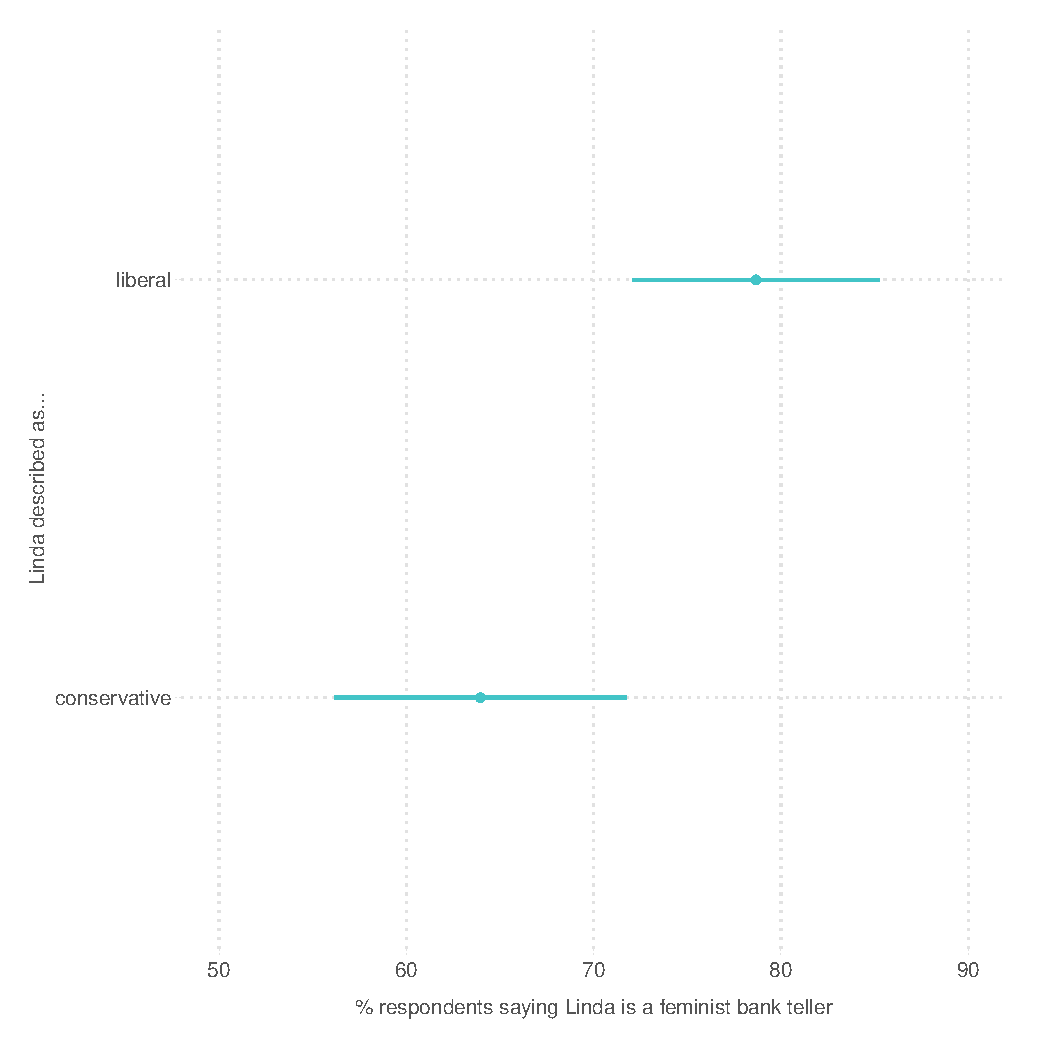
\includegraphics[width=1\textwidth]{../figs/linda_gg.pdf}
\end{center}
\scriptsize{\textbf{Note}: Point estimates shown with 95\% confidence intervals.}
\end{figure}

On the other hand, it is worth noting that even in the {\tt conservative} condition---from which one might reasonably infer that Linda is pro-life---65\% of respondents in the MTurk study committed the conjunction fallacy. Two distinct explanations exist. Perhaps in a post-2016 climate, the ``philosophy major'' cue triggers imagery of liberal academics in ivory towers \citep[e.g.,][]{pew_education}. It seems more likely to us---again, given the contemporary political climate---that people attribute feminism to women active on \emph{any} political issue, but the data here cannot parse these two possibilities. What is clear, however, is that the patently counter-stereotypical policy cues reduced respondents' tendency to commit the conjunction fallacy---but not enough to lead a majority to correctly identify that Linda must be a bank teller if she is also a bank teller active in the feminist movement. In sum, the lingering social cues, beyond those policy cues provided, appeared quite powerful.

\subsection{Experiment 2: James, a man of many identities}

Our manipulation of Linda demonstrates that representativeness contributes to political stereotyping: when given information about someone or something representative of a political group, people will jump to conclusions---even if the conclusion is logically impossible. With a new character named James, we build on this finding two ways. First, we demonstrate that this tendency extends to party stereotyping, the particular form of political inference in which we are interested. Second, we assess the degree to which people home in on various characteristics when inferring partisanship, which allows us to gauge whether those which are most representative also most yield stereotyping. The wording for the initial ``James Problem'' is as follows:
\begin{quotation}
\noindent James is a 37-year-old (white | Black) man. He attended the University of Michigan, where he double-majored in economics and political science and was president of a business and marketing club. 
\vspace{0.1in}

\noindent James's co-workers describe him as highly driven, outspoken, and confident. He is married to (Karen | Keith), whom he met in college, and they have one son. In James's free time, he (leads his son's Cub Scouts group, organized through the Baptist Church the family attends | leads his son's Junior Explorers group, organized through the secular parents' network that the family belongs to | coaches his son's youth sports teams).
\vspace{0.1in}

\noindent Which of the following is most likely?
\begin{itemize}
\item James works in sales
\item James works in sales and is an active supporter of the Democratic Party
\item James works in sales and is an active supporter of the Republican Party
\end{itemize}
\end{quotation}

We thus manipulate three characteristics related to James's social group memberships: race, sexual orientation, and religion. In the case of religion, we have a control cue. Instead of James leading his son's scouting group organized through a religious or secular organization, ``James coaches his son's youth sports teams.'' In our first iteration of the James experiment, conducted on MTurk in January 2018 $(n=297$), we provide \emph{maximal contrast}: we randomly assign respondents to a purely Democratic-representative James, a purely Republican-representative James, or a control James who is white and straight (as are a majority of Americans) with the ``youth sports'' cue provided instead of a religious one. 

If representativeness drives party stereotyping, in the maximal contrast experiment we should observe the Democratic conjunction fallacy most clearly in the Democratic-representative condition (and hardly at all in the Republican-representative condition), and we should observe the opposite in the Republican-representative condition. We compare responses in both of these conditions to those in the control condition.

Our second iteration of the James experiment is \emph{fully factorial}: James's characteristics vary randomly and independently within the vignette. For example, a respondent may encounter a white, gay, sports-coaching James. This allows for inferences about which characteristics most push respondents toward the conjunction fallacy, which in turn allows us to better illuminate the relationship between representativeness and stereotyping. To this end, we increase the dimensions on which James may vary, specifically including variation on policy preferences. At the end of the first paragraph we insert the sentence: ``He also participated in (anti-tax demonstrations | living-wage demonstrations | student government).'' %This allows us to assess whether social identities are merely heuristics for gauging someone's policy preferences, which are used in turn to assess partisanship---or whether people consider social identities other ways.


\subsubsection{A comparison of maximal difference}

If representativeness bias fuels stereotyping, then the probability of committing party-specific conjunction fallacies ought to vary systematically as a function of how James is described. This is exactly what we observe in the first James experiment. When James is described as a gay, Black, secular man, 65\% of respondents erroneously report that he is most likely to be a Democratic salesman (as opposed to a salesman). Similarly, when James is straight, white, and Baptist, 62\% say that he's most likely to be a Republican salesman. Importantly, as Figure \ref{fig:James} shows, just a small minority of respondents in the Democratic (Republican) condition commit the Republican (Democratic) error, suggesting that representative traits lead people to systematically illogical conclusions.

\begin{figure}
\caption{Party-representative descriptions cause party-specific conjunction fallacies in the maximal-contrast ``James'' experiment}
\label{fig:James}
\begin{center}
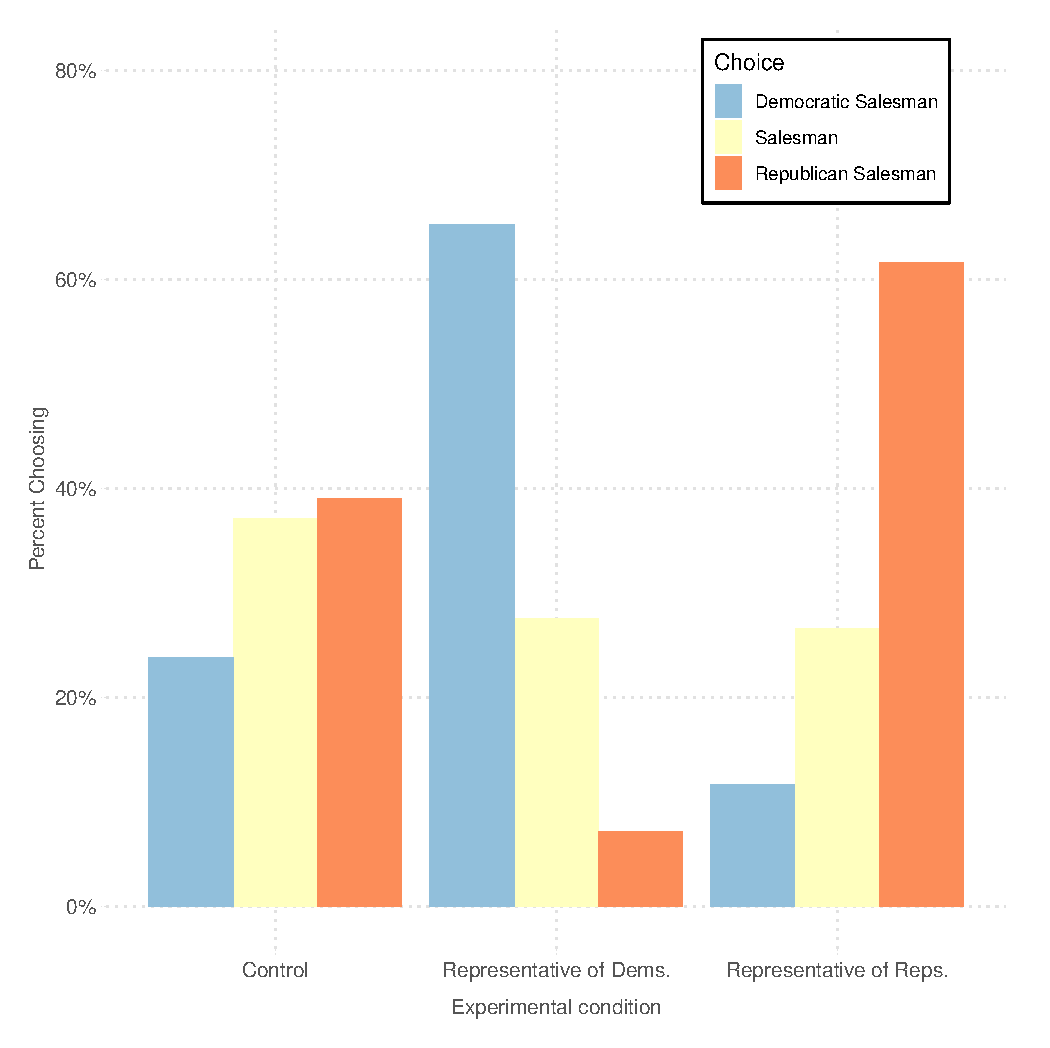
\includegraphics[width=1\textwidth]{../figs/fig_2_mturk_prop_by_treat_party_rep.pdf}
\end{center}
\end{figure}

Perhaps just as important, when James is less obviously representative of one party, people are less likely to commit the conjunction fallacy. Respondents in the control condition were 10 percentage points more likely to simply describe James as a salesman than those assigned to a party-representative condition $(p=.07)$. It is worth noting, however, that fewer than 40\% of respondents selected the correct answer. Even further, a small (and statistically insignificant) plurality of respondents in the control condition ascribed Republican support to James. We suspect this is because two of the three traits in the control condition were consistent with those in the Republican condition. Even if whiteness and heterosexuality (and being male, for that matter) are highly common in both the Democratic and Republican mass parties, they are somewhat representative of Republicans---perhaps especially so, post-2016.\footnote{It is also possible that being a salseman may be somewhat stereotypically Republican, as a business career.} This does not make respondents' conclusions correct---a logical error is a logical error---but it does potentially explain the somewhat anomalous result in the control condition. To better evaluate this possibility, we turn to a design that allows James's distinct characteristics to vary independently.

\subsubsection{A fully factorial design}

We conducted our second study on MTurk in August 2018, recruiting 1,991 respondents. Because of concerns raised about MTurk data quality that summer \citep[e.g.,][]{bai_2018, ryan_2018}, we implemented a filtering protocol consistent with \citet{ahler2019turk_nyu}, based on data collected pre-treatment, to weed out responses from foreign and Blacklisted IP addresses and insincere respondents \citep[e.g.,][]{lopezhillygus_2018}. The resultant sample includes $n=$ 1,507 respondents.\footnote{See SI 2 for further details on the filtering protocol.} 

As described above, we exposed these respondents to the ``James'' vignette but allowed four factors---James's race, sexual orientation, religion, and, new to this version of the vignette, a clue about his policy views---to vary randomly and independently. As such, we can estimate the \emph{average marginal component effect} ($AMCE$) of each independently randomized characteristic on the predicted probability of committing the Democratic and Republican conjunction fallacies. Since the dependent variable takes on three values---Democratic conjunction fallacy (-1), logically correct response (0), Republican conjunction fallacy (1)---we use an ordered logit model (omitting one value per variable) to analyze the data. Thus, our model takes the following form, with $i$ indexing respondents and $j$ indexing possible values of the dependent variable:

\begin{equation}
p_{ij} = p(y_{i} = j) =
    \begin{cases}
p(y_{i} = -1) = p(y_{i}^{*} \leq \alpha_{-1}) \\
p(y_{i} = 0) = p(\alpha_{-1} < y_{i}^{*} \leq \alpha_{0}) \\
p(y_{i} = 1) = p(\alpha_{0} < y_{i}^{*})
    \end{cases}
\end{equation}

\noindent where $y^{*}_{i}$ is the respondent's latent outcome and $\alpha_{-1}$ and $\alpha_{0}$ are the model's cutpoints. We model these probabilities as follows:

\begin{equation}
p(y_{i} = j) \sim \text{logit}^{-1}(\beta_{k}X_{ik} + \varepsilon_{i})
\end{equation}

\noindent where $X_{k}$ denotes our treatment vector---James's race, sexual orientation, religion, and policy views. Importantly, because these treatments were assigned randomly and independently of each other, $\beta_{k}$ captures the unique effect of attribute $k$, on average and independent of all other treatments in $K$. So even if James's sexual orientation could contribute to perceptions of James's religion, beyond what's provided in the vignette---as one example of how cues might interact---our design and model allow us to estimate the average marginal treatment effect ($AMCE$) of each cue provided, independent of the effects of the other cues \citep{hainmueller2013causal}. We can thus compare the magnitudes of these $AMCE$s to glean the cues most likely to lead to party-specific conjunction fallacies.

Full model results are available in SI 3. For ease of interpretation, we convert the resultant logit coefficients to the marginal change each randomly assigned treatment contributed, on average, to respondent $i$'s predicted probability of making the Democratic and Republican conjunction fallacies. We show these average marginal component effects in Figure \ref{fig:james_ff}.\footnote{Alternatively, we present the results as the simple marginal probabilities of committing the Democratic and Republican conjunction fallacies for each attribute in SI 3.1. Interestingly, as these results show when broken out by partisanship, Democrats and Republicans make these errors at about the same rates for each party, but independents are significantly less likely to commit the conjunction fallacy for every party-group pairing.} 

The results suggest that all of these cues significantly affect citizens' judgments about others' partisanship---to the degree that each, independent of the others, appears to lead people to reach the logically impossible conclusion that James is more likely to be a Democrat or Republican \emph{in addition to} being a salesman than he is to be a salesman. For example, regardless of how else James is described, if he is said to be Black, respondents are nearly 14 percentage points more likely to make the Democratic conjunction fallacy and nearly 10 points less likely to make the Republican one. All cues are not created equal, however. James's race and sexual orientation appear to make respondents significantly more likely to commit a party-representative logical conjunction fallacy than do James's religion or cues about his ideological leanings ($p < .10)$. This suggests that we may be just as liable, if not more so, to attribute partisanship to another individual on the basis of ascribed characteristics than on the basis of expressed policy views. 

\begin{figure}
\caption{Party-representative traits induce party-specific conjunction fallacies in the fully-factorial ``James'' experiment}
\label{fig:james_ff}
\begin{center}
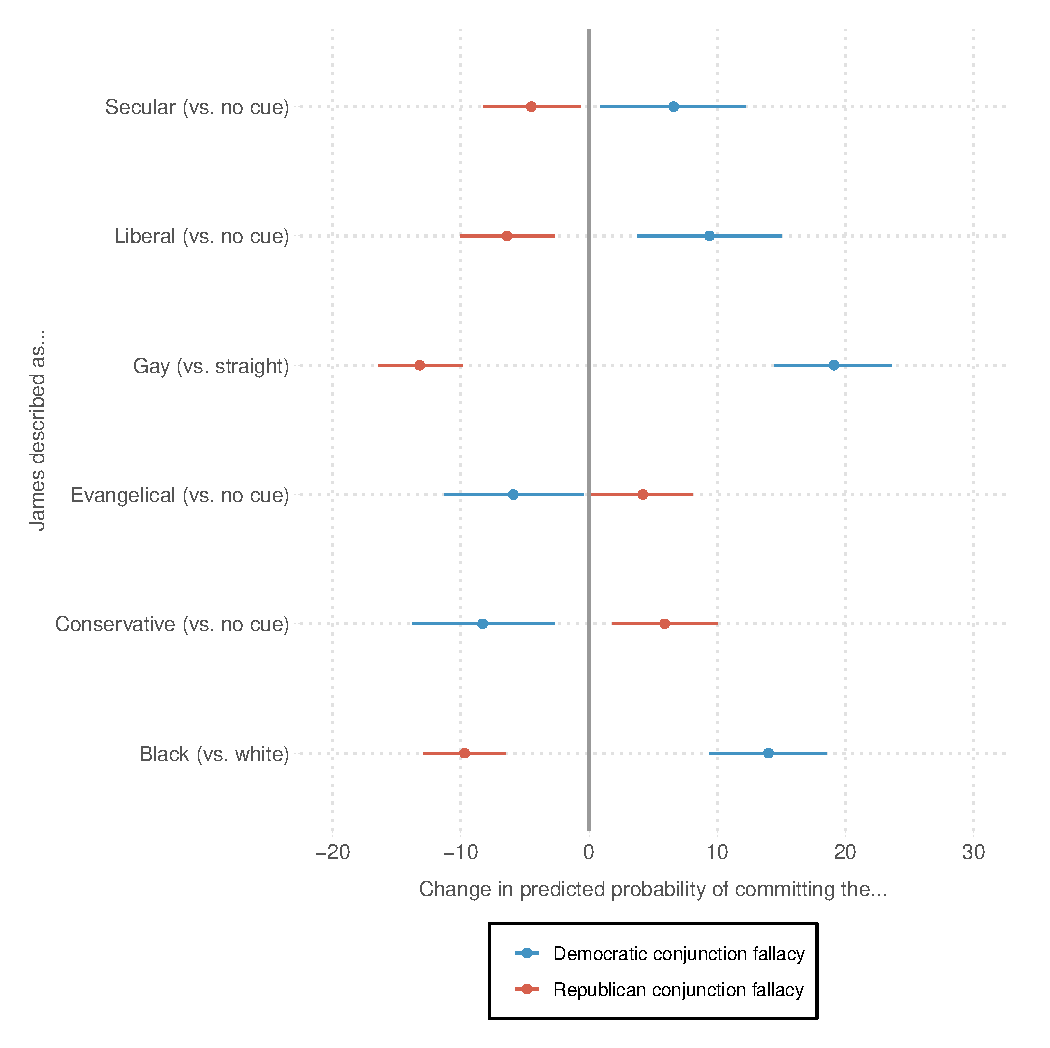
\includegraphics[width=1\textwidth]{../figs/james_ff.pdf}
\end{center}
\scriptsize{\textbf{Note}: Point estimates shown with 95\% confidence intervals.}
\end{figure}

Of course, this may not reflect a social--policy distinction as much as representativeness. Black Americans support Democratic candidates at a roughly 90\% rate, as do over 80\% of LGBT Americans \citep{fitzsimmons2018record}. By contrast, while secular and evangelical groups sort heavily into ``their'' parties, they do so at rates lower than these \citep{pew_religion} and, according to the most recent American National Election Study\nocite{ANES}, only three-quarters of Americans correctly identified the Republican presidential candidate as more conservative on taxes than the Democratic candidate. This pattern is worth noting but not reading too heavily into. It may be that more representative cues lead to greater party-stereotyping and, thus, to the conjunction fallacy at higher rates in this study. But it could also be that social cues are generally more powerful, or this result might simply reflect the cues chosen in this particular experiment. 
%Even if such cues about policy have a greater effect on affective partisan polarization \citep[e.g.,][]{orr2018measured, webster2017ideological}, people arrive at their conclusions about the typical partisan's policy views through their perceptions of what the party ``looks like'' \citep{ahlersood_2018}. At least in this case, race and sexual orientation appear more connected to partisanship than do 

%Taken together, both versions of the ``James'' experiment, as well as our extension of ``Linda,'' provide support for Hypothesis 3: the representativeness heuristic can lead folks reach illogical but stereotype-consistent conclusions, consistent with \citet{tversky1983extension}. But these exercises have been quite academic---while they demonstrate that representativeness \emph{can} lead to stereotyping of the sort that appears to drive partisan polarization \citep{ahlersood_2018}, does it actually do so? That is, aside from causing erroneous responses to contrived logic problems, does using the representativeness heuristic to divine what the parties ``look like'' lead to perceptual bias?


\section{Providing Bayesian Cues}

Linda and James confirm that the representativeness heuristic can lead people to illogical but prototype-consistent conclusions. They further show that people use this type of reasoning to infer others' political characteristics, regardless of cues that appear relatively obvious (in this case, illogical conjunctions) and that should suggest more tentative judgments. With a second design, we more thoroughly investigate the degree to which people use the cues that Bayes's Theorem says they should---or don't use them, as Equation \ref{eq:rep} and H2 suggest may be the case.

We randomly assigned respondents to one of three conditions in a survey experiment conducted on MTurk in the summer of 2016 $(n=911)$ before asking all for their perceptions of the shares of stereotypical groups in the Democratic or the Republican Party. We informed a random third of respondents about the shares of two party-stereotypical groups within ``their'' party, $p\text{(party | group)}$. This {\tt group composition} condition presents the type of information that polling reports convey about how groups sort into parties. To another random third, we presented information about the shares of party-stereotypical groups in the population, $p(\text{group})$. We label this treatment arm the {\tt base rates} condition. The remaining third received no information and serves as our {\tt control} group.

In the information provision conditions, we first asked respondents either for their perceptions of the groups' base rates or the shares of those groups that identify with the party to which they are stereotypical. (So, for example, those in the Democratic {\tt base rates} conditions were asked for their perceptions of the percentage of American adults who are union members or who identify as gay, lesbian, or bisexual.) We then gave respondents the corresponding correct statistics through a cover story. We said, ``...As part of our study on people's ability to remember numbers, we will re-quiz you on these at the end of the survey. If you answer the re-quiz questions correctly, you will receive a 10-cent bonus through MTurk within a week.'' The critical design feature is that we expected respondents to write this number down, or at least keep it at the top of their heads, so that it would be unusually accessible. After providing these quantities, we asked respondents a series of unrelated questions. We quizzed them about the provided statistics immediately before we elicited their perceptions of $p(\text{group | party})$, the dependent measures. (See SI 1.2 for a visual depiction of the survey experiment.) In the {\tt base rates} condition, 93.6\% of respondents recalled the correct number. In the {\tt group composition} condition, 93.4\% did. All respondents, including those who couldn't recall the right number, were presented with the correct information again immediately after the quiz.

Our dependent variable is the perceived share of party-stereotypical groups in either the Democratic or the Republican party. The Democratic battery included questions about the percentage of Democrats who are gay, lesbian, or bisexual (6.7\% according to the 2012 ANES) and the percentage who are union members (11.1\%). The Republican battery included perceptions of the percentage of Republicans who earn over \$250,000 per year (2.0\%) and who are evangelical Christian (34.3\%). Respondents assigned the Republican battery were provided information about Republican-stereotypical groups, and those assigned to the Democratic information were provided information about the Democratic-stereotypical groups. The base rates of the groups we provided information about are as follows: 3.8\% of adult Americans are gay, lesbian, or bisexual, 11.3\% belong to a union, 19.1\% are evangelical, and 2.0\% earn at least \$250,000 per year (again according to the 2012 ANES). The group composition information we provided is as follows: 63.1\% of the LGBT and 41.9\% of the union members identify as Democrats and 56.1\% of evangelical Christians and 49.7\% of those who earn at least \$250K identify as Republicans.\footnote{Some have challenged the validity of these statistics, asserting that they are either underreports for some groups or that the 2012 numbers were underreports for 2016, especially because of increasing party sorting \citep[e.g.,][]{Levendusky2009}. Even if true, our interest here is not in eliciting responses to the exact statistics, but rather how respondents react to different \emph{types} of statistical cues---in this case, base rates $p(\text{group})$ and inverse probability $p\text{(party | group)}$---vis-a-\`{a}-vis pure intuition. One might be concerned about treatment compliance---i.e., respondents may not have believed the information if they thought some statistics were wrong---but, if so, this concern should bias results against treatment effects.}

Since representativeness, taken to the extreme, implies equating $p\text{(party | group)}$ with $p(\text{group | party})$, we expect providing information about $p\text{(party | group)}$ will make reported perceptions of $p(\text{group | party})$ closer to the former. In short, and consistent with H1, we expect greater bias in the {\tt group composition} condition. 

As per H2, we expect that the {\tt base rates} condition will have little effect on the elicited perceptions. On the other hand, since we incentivized learning and recall, the treatment may have a greater impact than previous base rate treatments \citep[e.g.,][]{ahler2018parties}. 

\citet{sides2007b} suggest that the innumerate may rely on representativeness more. To investigate this possibility and assess H4, we measured numeracy. We administered a four-item battery to assess respondents' skills with percentages, probabilities, and numerical quantities more generally (see SI 1.2.2 for the individual items) and rescaled this index 0--1. First, like \citet{sides2007b}, we expect the less numerate to have more biased perceptions. Second, if people use representativeness heuristically when envisioning the parties, we expect the least numerate to be most influenced by the {\tt group composition} treatment.

\subsection{Results}

Consistent with reliance on representativeness, people appear to conflate $p(\text{group | party})$ with $p(\text{party | group})$. As Figure \ref{fig:rep_ciplots} shows, for three of the four party-group dyads, participants primed to consider {\tt group composition} by partisanship report yet-more inflated estimates of those groups' shares in ``their'' parties. The one dyad for which this is not the case is the Democratic-union dyad, the pairing for which the group is least representative of ``its'' party---just 41\% of union members are Democrats. Not only do we find support for our first hypothesis, but we find further piecemeal evidence, consistent with that from the fully factorial ``James'' experiment, that representativeness fuels stereotyping. 

Interestingly, and contrary to Hypothesis 2 and previous work in this vein, providing base rates does appear to reduce perceptual bias. As shown in Figure \ref{fig:rep_ciplots}, respondents who were given base rates and incentivized to remember them perceived significantly fewer stereotypical partisans, on average, for three of the four party-group dyads. The one for which this is not true is the Republican-evangelical dyad, the pairing for which the group is most common in the population and for which respondents' estimates of the group's base rate were most accurate.\footnote{The average estimate of $p$(evangelical) was 27\%, off by roughly 8 percentage points. Respondents failed to come within ten points of the truth, on average, for none of the other party-stereotypical groups.} This pattern suggests that respondents may attend to base rates when assessing $p(\text{group | party})$, but only when their attention is unusually directed toward the base rate or they face incentives. The discrepancy with the Republican-evangelical dyad, however, suggests that base rate corrections may only matter when people misperceive the group's base rate by a large quantity.

\begin{figure}
\caption{When people focus on $p(\text{party | group})$, party stereotyping worsens}
\label{fig:rep_ciplots}
\begin{center}
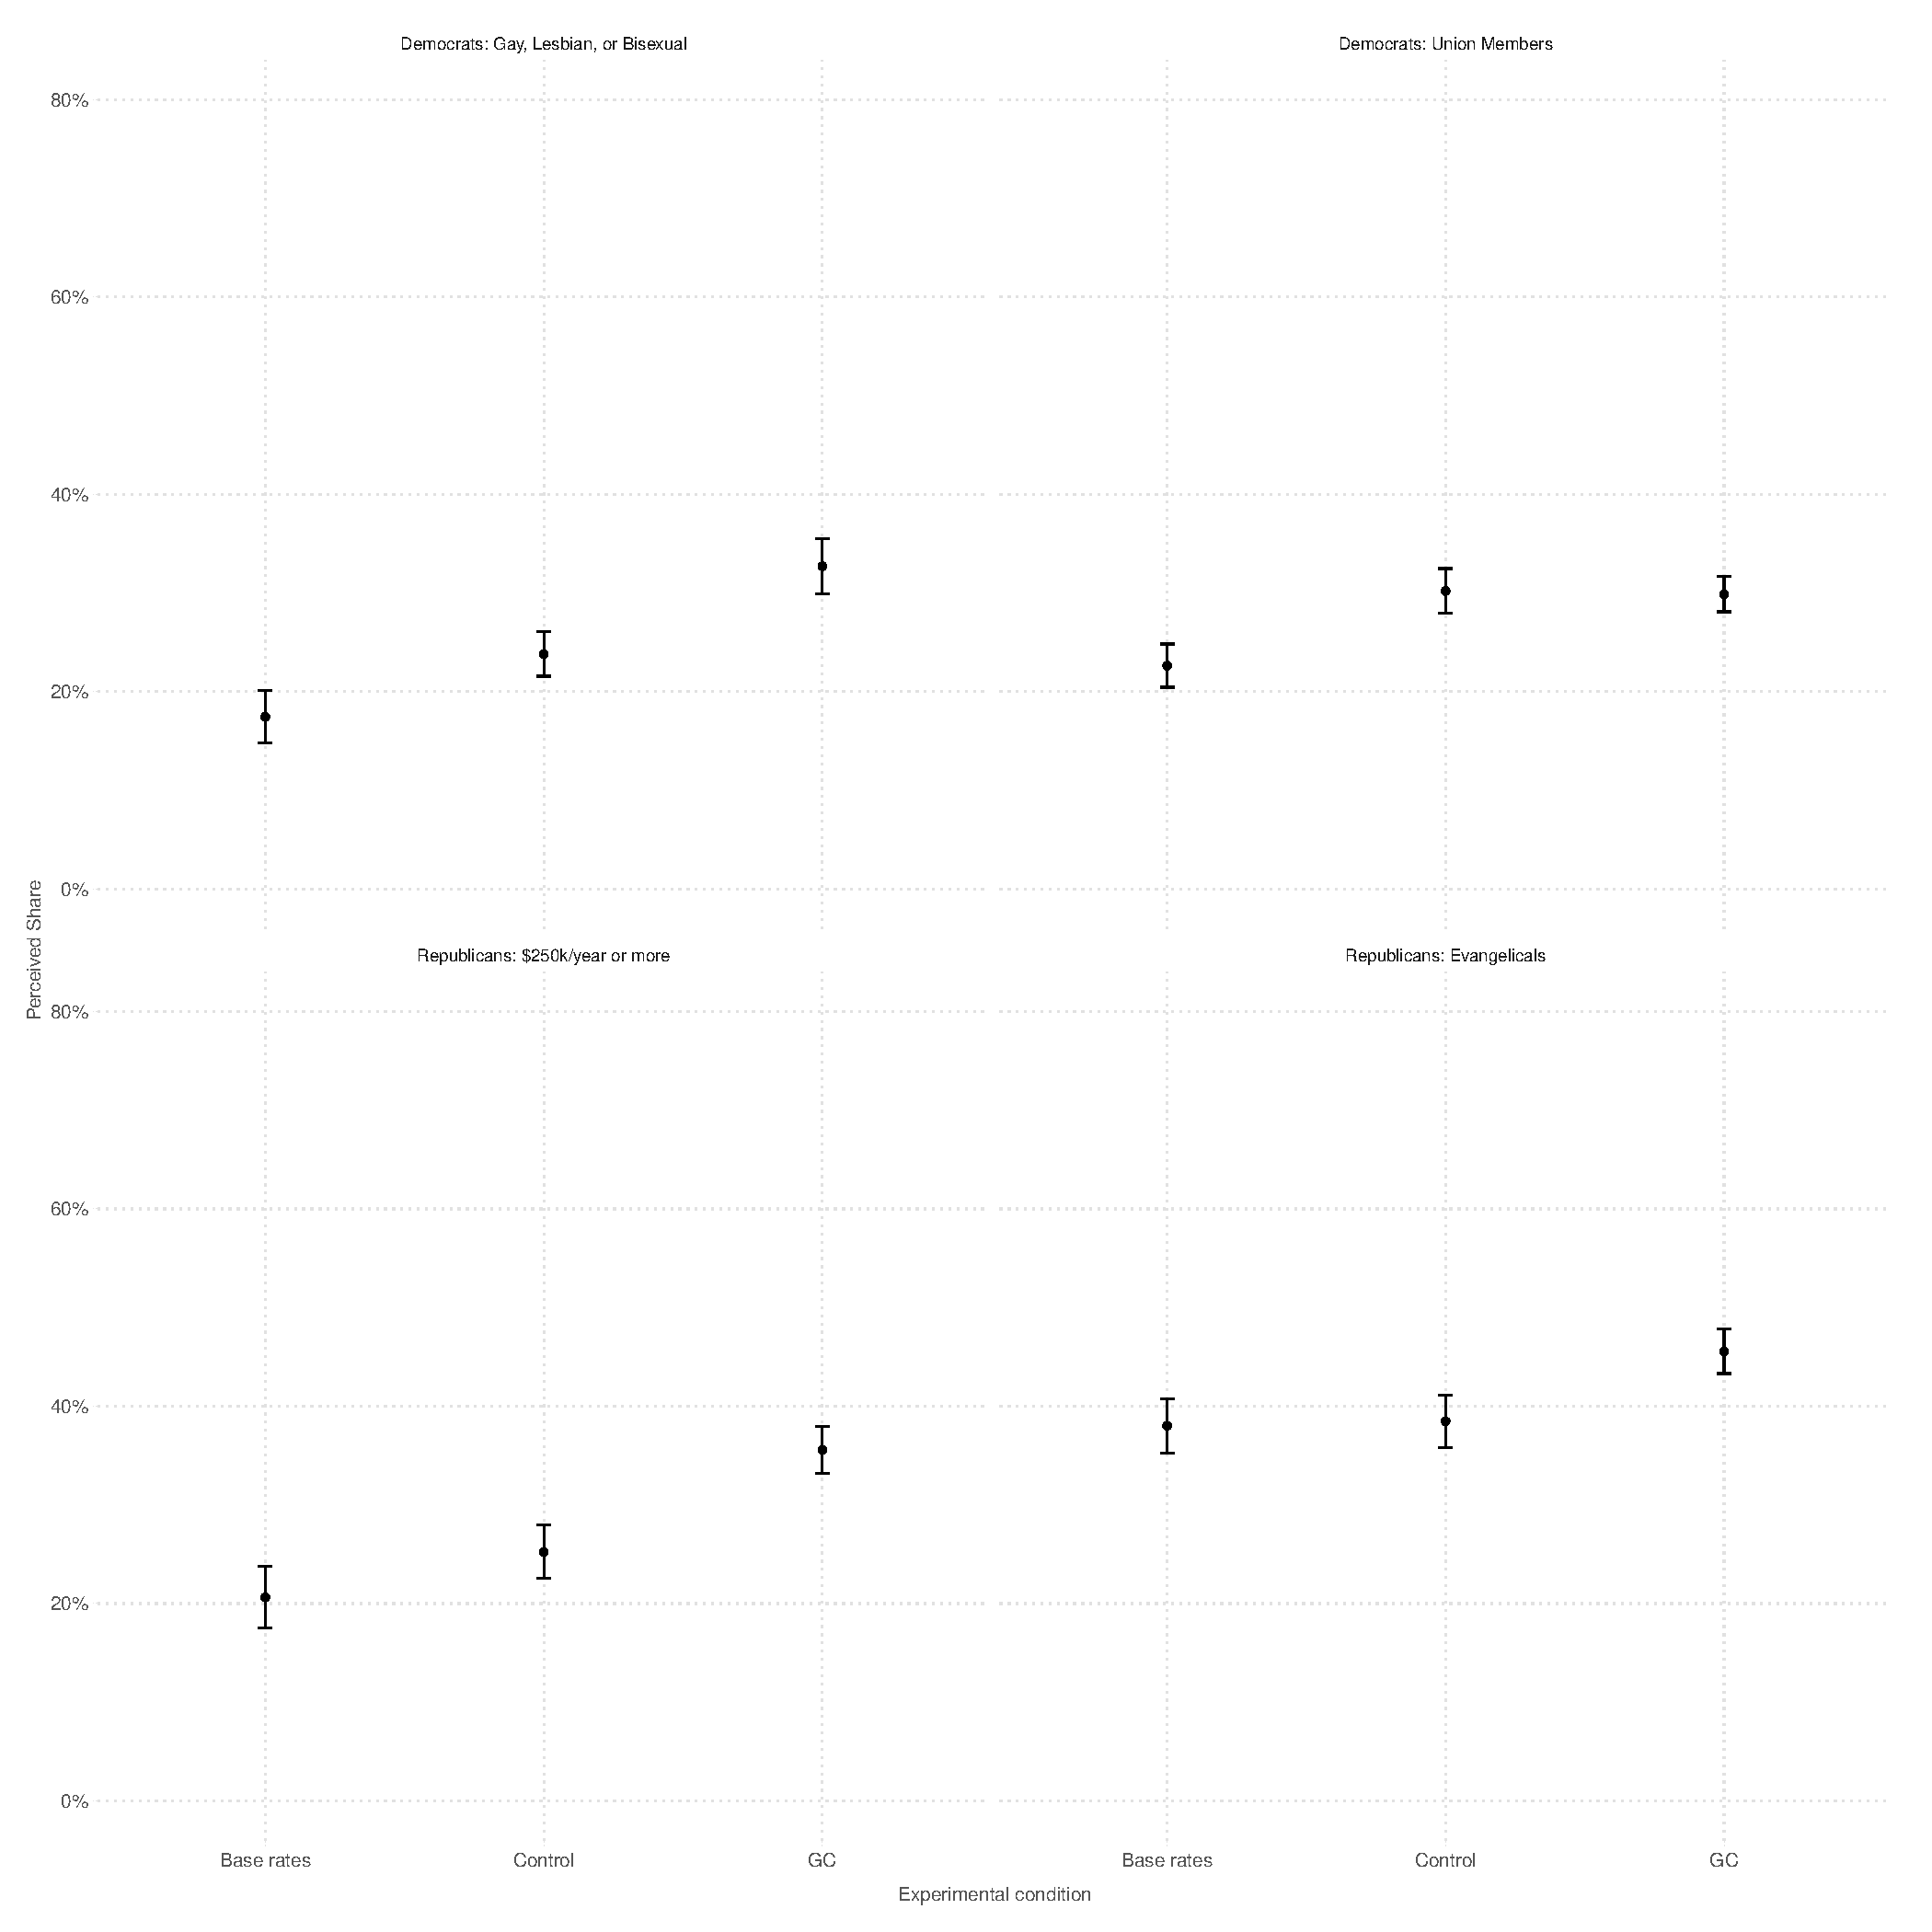
\includegraphics[width=1\textwidth]{../figs/misinfo_bayes_fig.pdf}
\end{center}
\end{figure}

Table \ref{tab:representativeness} summarizes the comparisons in Figure \ref{fig:rep_ciplots} with linear regression (OLS). We stack the data at the respondent-perception level and regress perceptions of $p(\text{group | party})$ on indicators for treatment assignment, including fixed effects for particular party-group dyads and clustering standard errors by respondent. As column 1 shows, the {\tt base rate} treatment reduces perceptual bias by five points, on average, while the {\tt group composition} treatment increases perceptual bias by 7 points. 

As one would expect, those who are more comfortable with probabilities and percentages hold less biased perceptions of $p(\text{group | party})$. Pooling across items, including fixed effects for items and clustering standard errors by respondent, the most numerate respondents are 13.8 points less biased in their perceptions, on average than the least numerate respondents (who err by 29.5 points; this comparison lacks the controls for experimental conditions in Table \ref{tab:representativeness}).

\begin{table}[]
\caption{Representativeness and innumeracy cause people to over-apply party stereotypes}
\label{tab:representativeness}
\begin{center}
\begin{tabular}{l|cc|}
\cline{2-3}
                                                  & \multicolumn{2}{c|}{DV: Reported Perception of $p(\text{group | party})$} \\ \cline{2-3} 
                                                  & (1)                             & (2)                             \\ \hline
\multicolumn{1}{|l|}{Numeracy}                    &                                 & -0.10***                        \\
\multicolumn{1}{|l|}{}                            &                                 & (0.04)                          \\
\multicolumn{1}{|l|}{Base rate treatment}         & -0.05***                        & -0.07                           \\
\multicolumn{1}{|l|}{}                            & (0.02)                          & (0.05)                          \\
\multicolumn{1}{|l|}{BR X numeracy}               &                                 & 0.03                            \\
\multicolumn{1}{|l|}{}                            &                                 & (0.06)                          \\
\multicolumn{1}{|l|}{Group composition treamtent} & 0.07***                         & 0.25***                         \\
\multicolumn{1}{|l|}{}                            & (0.02)                          & (0.04)                          \\
\multicolumn{1}{|l|}{GC X numeracy}               &                                 & -0.23***                        \\
\multicolumn{1}{|l|}{}                            &                                 & (0.05)                          \\
\multicolumn{1}{|l|}{}                            &                                 &                                 \\
\multicolumn{1}{|l|}{Constant}                    & 0.29                            & 0.37                            \\
\multicolumn{1}{|l|}{}                            & (0.01)                          & (0.03)                          \\
\multicolumn{1}{|l|}{$R^{2}$}     & 0.11                            & 0.15                            \\
\multicolumn{1}{|l|}{SER}                         & 0.22                            & 0.22                            \\
\multicolumn{1}{|l|}{$n$ respondents}             & 911                             & 911                             \\
\multicolumn{1}{|l|}{$n$ perceptions}             & 1822                            & 1822                            \\ \hline
\end{tabular}
\end{center}
\end{table}

As perhaps our clearest evidence that the representativeness heuristic fuels party stereotyping, the {\tt group composition} treatment appears to affect the least numerate respondents the most. In column 2 of Table \ref{tab:representativeness}, we observe a large, negative, and significant interaction effect of the {\tt group composition} treatment and scores on the numeracy battery. This interactive effect is nearly identical in absolute magnitude to the also-significant but \emph{positive} main effect of the {\tt group composition} treatment. This implies that the least numerate respondents are strongly affected by the treatment---they inflate their estimates of $p(\text{group | party})$ when given $p(\text{party | group})$---but that the most numerate respondents are not. This is consistent with using heuristics \citep{kahneman1972subjective}: those need the most help depend the most on the provided ``shortcuts.'' The {\tt base rates} treatment, on the other hand, does not appear to give rise to an analogous interactive effect: all respondents appear equally likely to use the base rate cue to reduce bias, although this apparent substantive effect is no longer statistically significant in the fully-specified model.

Thus, we find clear evidence for H1: when provided, people will rely unduly on the share of group $g$ that supports party $p$ to judge party composition. Consistent with representativeness, the one group-party dyad for which we do not observe this pattern is the union-Democratic pairing---the only one in which a clear minority of group members (albeit still a plurality) supports the party. We observe this judgment shortcut primarily among less numerate respondents, providing support for H4. Finally, we find mixed support for H2---that people will ignore base rates, even when provided. Contrary to past studies, respondents adjusted their perceptions of $p(\text{group|party})$ downward when they received group base rates. But two nuances are worth noting. First, because of our design, respondents were unusually attuned to these quantities. Second, although we observe similar main effects of the {\tt group composition} and {\tt base rates} treatments, their interactive effects with respondent numeracy belie different data-generating processes. Those who most ``need help'' with their back-of-the-envelope calculations about the percentage of Democrats who are LGBT, for example, most rely on the given percentage of LGBT Americans who support the Democratic Party---the very types of cues often provided in media analyses of polling data. We do not observe low-numeracy respondents similarly reaching for the provided base rates. Thus, although we only find mixed support for H2, the Bayesian cues experiment demonstrates how uniquely attuned we are to representativeness when making judgments about how groups compose other groups. In this sense, we are hard-wired to perceive polarization. 

\section{Forcing Snap Judgments to Reveal the Representativeness Heuristic}

People likely do not walk around with concrete beliefs about the percentages of the Democratic and Republican parties belonging to various groups. Instead, we suspect they hold fuzzy beliefs about party composition, based on their party prototypes, which map to the actual numbers they report on surveys \citep{ahler2017}. If this is the case, and people use representativeness heuristically to assess the composition of the parties, then we ought to observe differences in perceptual bias under different cognitive constraints. More concretely, and consistent with H4, we expect that people facing time pressure when making these judgments will more strongly rely on representativeness and thus show greater bias in their beliefs about how party-stereotypical groups compose ``their'' parties.

We conducted an experiment on MTurk $(n=284)$ in Summer 2016 to assess whether cognitive load, operationalized as pressure to respond quickly, leads people toward more biased judgments about party composition. Respondents were randomly assigned to one of two conditions: a {\tt time pressure} condition in which they had to answer each of four randomly chosen party composition questions (like those in the Bayesian cues experiment) within ten seconds, or a {\tt time requirement} condition in which they had to wait fifteen seconds to respond to each question (with the question text, but no response box, on-screen). If heavy cognitive loads lead people to rely more heavily on representativeness, then respondents in the {\tt time pressure} condition should report more biased perceptions.

\subsection{Results}

Indeed, this is the pattern we observe. Reshaping the data so that each row is one of each respondent's four reported perceptions, we regress (via OLS) respondents' numerical perceptions on an indicator for the {\tt time pressure} condition, including fixed effects for each unique party-group dyad and clustering standard errors by respondent. All else equal, respondents facing {\tt time pressure} reported beliefs about party composition that were 5.8 percentage points more biased $(p=.01)$; see Figure \ref{fig:timing}). This difference cannot completely explain misperception---as \citet{ahler2018parties} note, people tend to err by roughly twenty points when making these judgments. But along with the numeracy-related findings from the Bayesian cues study, this outcome demonstrates that cognitive load worsens perceptual error, consistent with using representativeness heuristically.

\begin{figure}
\caption{Perceptual bias worsens with cognitive constraints---consistent with using representativeness to heuristically infer party composition}
\label{fig:timing}
\begin{center}
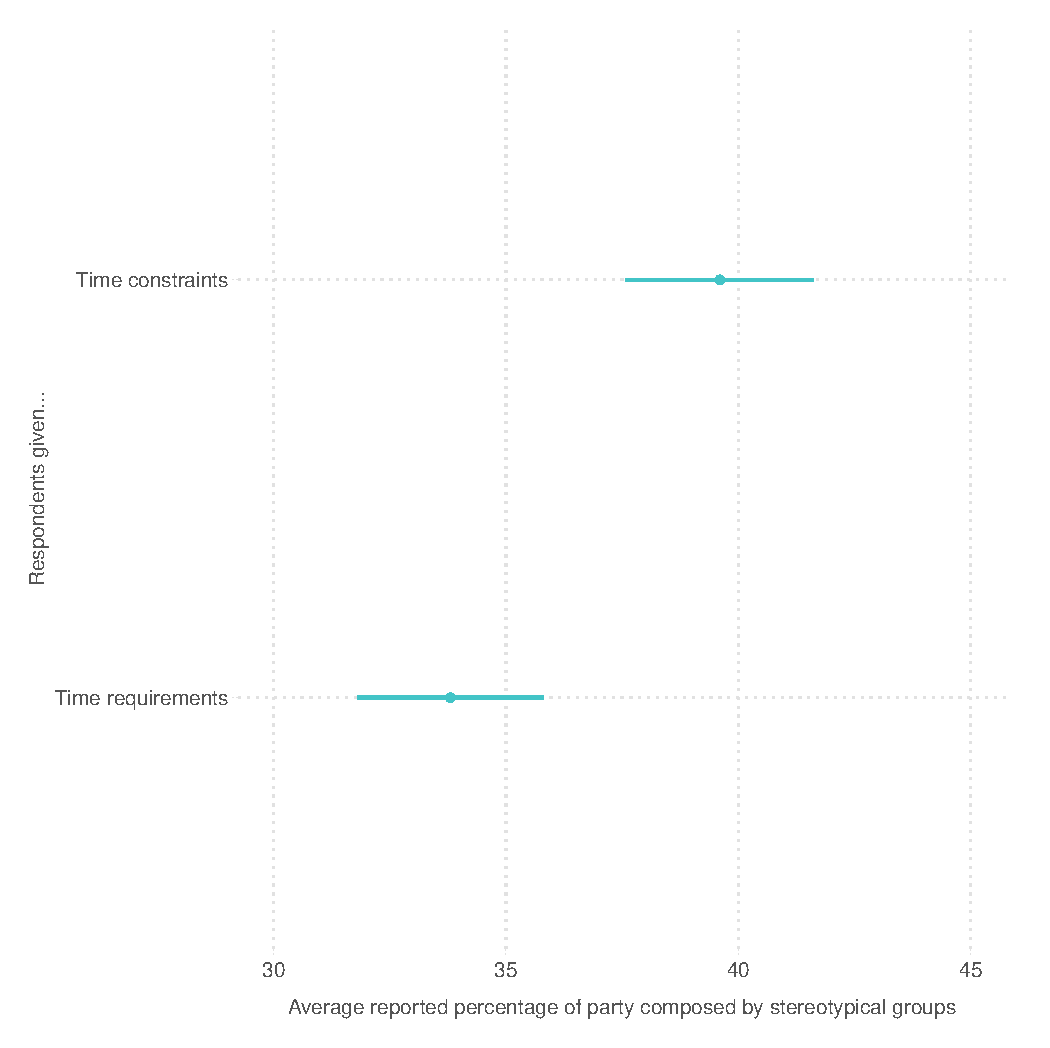
\includegraphics[width=1\textwidth]{../figs/timing.pdf}
\end{center}
\scriptsize{\textbf{Note}: Point estimates shown with 95\% confidence intervals. The average share of ``its'' party composed bv the 8 party-stereotypical groups is 17.9\%.}
\end{figure}

Cognitive capacity is limited, and public affairs aren't a priority for most. This is important for contextualizing these results. If most were political savants, then we'd expect their real-life judgments to be more like those of the most numerate in the Bayesian cues experiment, or like those reported under time requirements in this study. But most people direct their attention away from politics, only tuning in during major elections or unusual circumstances. Citizens often possess shallow images of the parties in general \citep{BullockEtAl2015, Converse1964, dancey2016inferences, DelliCarpiniKeeter1995, KuklinskiEtAl2000} and are woefully uninformed about the particular issue positions, priorities, or coalitions they champion \citep{Levendusky2010, Zaller1992}. As a consequence, we suspect that most people form party stereotypes more in accordance with the {\tt time pressure} condition than its counterpart---heuristically, with few considerations, and, ultimately, from the gut.\footnote{See SI 4 for an example of this---even when we provide survey respondents with significant time requirements and the ability to study pictures of the hypothetical parties, they still respond with stereotypical reports.}

\section{Discussion}

In 2004, when sentiment between Democrats and Republicans seemed like it couldn't get worse, Dave Barry made a humorous attempt to get Americans to look past their differences: \nocite{barry2004nyt}
\begin{quotation}
\noindent Do we truly believe that ALL red-state residents are...NASCAR-obsessed, gun-fondling, religious fanatic rednecks; or that ALL blue-state residents are godless...latte-sucking, tofu-chomping, holistic-wacko, neurotic, vegan weenie perverts?
\end{quotation}
\noindent Although funny---because stereotypes do have a ring of truth to them!---Barry's query makes us laugh a little less after conducting this research. Americans' stereotypes may not be quite as biased as he implies, but they are bad enough to cause concern. That is, people don't think that ALL Democrats are the type of people who live in Berkeley or Cambridge, but they think that prototypical partisans compose ``their'' parties far more than they truly do. Even more importantly, these stereotypes affect how people evaluate parties, the positions they think the parties take, and how they feel toward the other side \citep{ahler2018parties}. 

Barry's prose reads more somber mainly because we now see how easily one can be lulled by the siren song of representativeness. It is easy to laugh in passing at the notion that all Republicans are stock car junkies, but it appears far more difficult to internalize that the parties aren't as distinct (at least socially) as our guts tell us. In a sense, we are hard-wired against doing so. Regardless of whether we are categorizing people into parties or comestibles into food groups, humans require mental architecture for quickly putting people or things into broader boxes. As cognitive misers, we draw the maximal difference between mutually exclusive categories so that this task is relatively easy \citep{RoschMervis1975}---rather than focusing solely on characteristics that describe most group members. That is, we \emph{typecast} members of heterogeneous groups to make sense of daily life.

The studies presented in this paper demonstrate that this process underlies political stereotyping of the sort Dave Barry lampooned. People arrive at statistically impossible judgments like the conjunction fallacy---e.g., to say its more likely that ``James works in sales AND is an active supporter of the Republican Party'' than ``James works in sales''---when confronted with someone with representative characteristics of a political group. When given information about the degree to which a group supports a particular party, the least quantitatively adept rely unduly on that cue when judging party composition, consistent with the representativeness heuristic. Similarly, people facing time pressure---and, thus, a heavier cognitive load---report perceptions of party composition even more biased toward the share of the group belonging to the party. Importantly, we do not observe the heuristic use of groups' base rates. Although people highly attuned to groups' base rates appear to use them when judging party composition, at least in our Bayesian cues experiment, we fail to observe the less numerate doing so systematically, as they do with cues about group composition by party. This suggests that people process these two pieces of information differently when judging party composition, and in a manner consistent with \emph{base rate neglect}: when trying to heuristically solve a tough problem about conditional probability $p(\text{A|B})$, people will rely on representativeness and focus on the inverse probability $p(\text{B|A})$ to the detriment of base rates $p(\text{A})$ and $p(\text{B})$ \citep{KahnemanFrederick2002}.

A corollary of our experimental findings, however, is that stereotyping is not immutable. Contra past studies, people's perceptions of party composition did improve somewhat when we made group base rates especially salient. Furthermore, when we required people to stop and think before reporting their perceptions of party composition, they became less biased. We suspect, though, that these conditions for reflection rarely occur for most folks. As \citet{Dahl1961} wrote, ``Politics is a sideshow in the great circus of life'' (p. 305). To the extent that people assess the accuracy of their mental maps, politics is unlikely to be a priority. This is especially the case in today's world, where politics is often communicated in 280-character tweets and single-photograph memes, and in which stories rarely make it 24 hours in the news cycle. Expedient political elites can---and do---use these communication strategies to appeal to their constituents' basest instincts, often reinforcing latent party-group stereotypes for personal or partisan electoral gain. %(ADD SI SECTION WITH EXAMPLES). 
Even news outlets without nefarious intentions may overstate partisan differences because conflict sells \citep{FiorinaAbramsPope2005,levendusky2016media}. We should not look to the political class to help citizens overcome their predispositions toward party stereotyping. But this doesn't mean tempering political stereotyping is a lost cause altogether, as even improving citizens' general competence with numbers and probabilities could improve their judgments about the political environment. More systematically, media literacy organizations ought to develop ways to get citizens the information they actually need to conceptualize the parties, so that they may avoid fumbling around with faulty cues. 

In particular, as people construct the mass parties in their heads, they may have seemingly helpful but potentially misleading cues at their disposal. Polling reports and media accounts of the electoral horse race often describe how groups in society sort into one party or the other---for example, the oft-cited statistic that 90\% of Black Americans vote for the Democratic Party \citep[e.g.,][]{tyson2018pew}. This type of information appears readily available to citizens through polling reports and media accounts of electoral politics \citep[e.g.,][]{baldassare2019ppic,edsall2019why,fitzsimmons2018record}, and these reports rarely provide information about how groups compose parties or those groups' base rates in the population. While it is true that the parties have sorted on many different dimensions over the past few decades \citep[e.g.,][]{Levendusky2009,mason2018uncivil}, the mass parties remain relatively similar in their composition---much more so than people believe \citep{ahler2018parties}. But, as the Bayesian cues experiment shows, these ubiquitous reports on groups' partisan composition can activate ``like goes with like'' reasoning---e.g., ``If 90\% of Blacks vote Democratic, a large share of Democrats must be Black.'' Without information about groups' base rates in the population, even the most numerate respondents are liable to conflate the cue available to them---how groups sort into parties---with the information they actually want---the shares of those groups in the parties. 

In this sense, media may polarize Americans in a more subtle way than previously examined. A great deal of work has hypothesized and documented a ``polarization narrative'' \citep{FiorinaAbrams2008, LevenduskyMalhotra2013, levendusky2016media}---the potential exaggeration of partisan polarization through the media. But even if the newsmakers aren't intentionally inflaming partisan passions directly as such, the way they report on politics and elections may still do so indirectly. That is, if people use the representativeness heuristic to infer party composition, the frequency with which they encounter information that ``X group voted for Y party at a rate of Z\%'' is liable to lead people to see parties that are far more stereotypical in composition than they truly are, thus fueling affective polarization. Providing even slightly more comprehensive information about group-party linkages---groups' base rates, for example---could potentially alleviate some of the most errant partisan stereotyping.

We will probably never eradicate stereotyping, political or otherwise. Without organizing our knowledge around simplified mental imagery, the world would be entirely too complex to process. Our goal, however, should always be to form better judgments that will help us to make better downstream decisions. We suspect that most Americans are all too willing to accept simplifications like ``all Democrats are muggles'' or ``all Republicans are Death Eaters'' without critically evaluating them, especially when thinking about the out-party. And the more we accept these simplifications, the more we internalize the ``us and them'' dynamic that leads to ill will and prejudice \citep[e.g.,][]{lepore1997category}. If we could find a way to make the question, ``Wait, does that actually describe the party very well, or is it just representativeness?'' just as automatic as blind acceptance, we might reduce people's tendency to paint all partisans with a broad brush. Although this seems like a tall order, our contemporary politics demand it.

\clearpage

\bibliographystyle{apsr}
\bibliography{typecast.bib}

\end{document}